\subsection{Logical View}

\begin{figure}[H]
	\begin{center}
		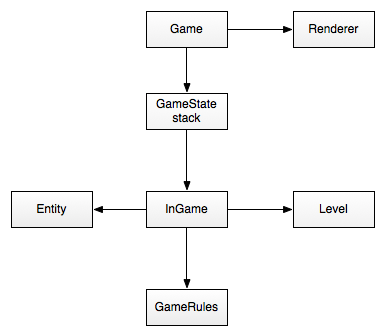
\includegraphics[scale=0.75]{graphics/DataManagementView}
	\end{center}
        \caption{Box and arrow diagram of game classes}
\end{figure}

The box and arrow diagram shows which modules and components that will be
used to implement the design. XNA assumes a Game class as the entry point of
the application, so this will be where everything starts. Aside from that,
we clearly need a DataManager to facilitate a data-driven application. The
idea here is that the DataManager will be able to import all kinds of data that
may be required by other components of the game, such as sprites, hero statistics,
levels and so on. It should also be able to store and retrieve a highscore list.

The GameState stack is how the game keeps track of what it should be doing right
now. For example, assuming the player pushes Start to pause the game, what should
happen is that a Paused state is pushed onto the stack, and then popped whenever
the player is done pausing. This is where menus and the like are handled.

We have decided that a Renderer is desirable, so that we can switch around on how
the graphics are handled at a later date. To facilitate this, we implement a
uniform interface for how an object can get itself rendered to the screen, and
an instance of a Renderer of some sort is passed down the call-chain down to the
entities that wish themselves to be rendered. In other words, this enables us to
not have to define how objects are Rendered in the objects themselves, and should
enable us to easily change graphical styles and the likes late in the development
cycle.

Ingame is the class that handles everything game-mechanical, directly or
indirectly. This is where the game-loop takes place. It has access to an Event
system, currently envisioned to incorporate an EventQueue class, and an Event
class. Ingame objects are allowed to push Events onto the EventQueue. Using
Events allows us to skip defining trigger methods of various kinds on all the
objects in the game, and makes the game semi-scriptable, enabling us to quickly
add different kinds of behaviour for creeps, projectiles and everything else.
Instead of having triggers then, the various objects have EventHandlers, if
they are so inclined.

Movable, collidable objects are Entities. Heros and creeps are subclasses
of this class, as is Particle, which has a slightly different behaviour.
\subsection{Process View}

\begin{figure}[H]
	\begin{center}
		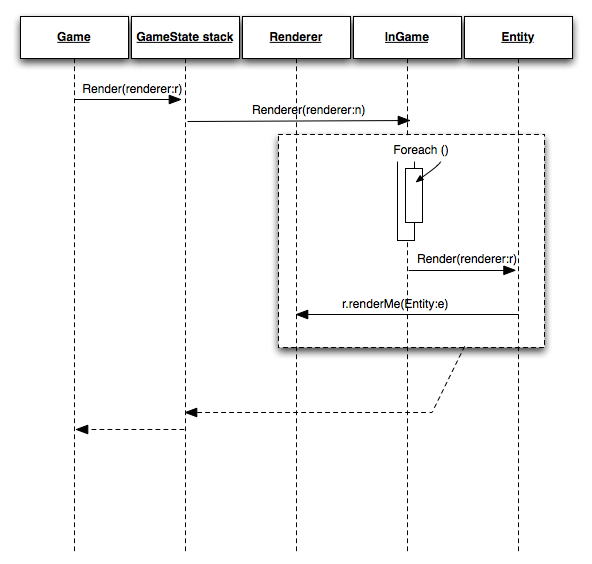
\includegraphics[scale=0.75]{graphics/GameRendersToScreen}
	\end{center}
        \caption{Game renders to screen}
\end{figure}

We have chosen to include 3 sequence diagrams that show the interactions between
components in some illustrative situations here. The first one shows how Rendering
of ingame objects takes place. The Game wants to render to screen, and so it
tells the GameState stack, and passes along a Renderer which it can use for this
purpose. The Game class does not need to be aware of which state the Game is in
to do this. The GameState stack knows that it is currently in a game, and so
it delegates this task to the Ingame class. This class iterates over all its
renderable objects, and tells them to render with the Renderer that was passed
down the call-chain. These then give the Renderer information about where they
are, and the Renderer does the rest.

\begin{figure}[H]
	\begin{center}
		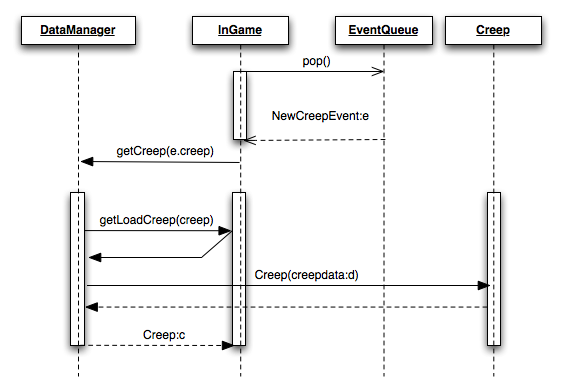
\includegraphics[scale=0.75]{graphics/GameSpawnsCreep}
	\end{center}
        \caption{Game spawns creep}
\end{figure}

The second one shows how creeps are spawned. At some point, a SpawnCreep event
was added to the EventQueue (Probably by the Level), and this event should now
be triggered as discovered by the EventQueue. Ingame polls the EventQueue,
and gets this event in return. It asks the DataManager for information about this
creep, and the DataManager discovers that it hasn't loaded this creep type yet, so
it has to fetch the data from the storage system. Once this is done, it
creates an instance of the creep type and sends it back to Ingame.

\subsection{Player Shoots}
\begin{figure}[H]
	\begin{center}
		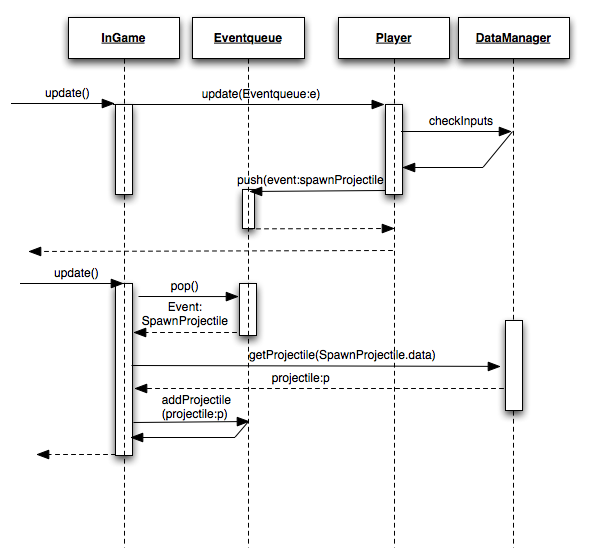
\includegraphics[scale=0.75]{graphics/PlayerShoots}
	\end{center}
        \caption{Player shoots}
\end{figure}

The third one details what happens when a player shoots. The essential of the
situation is that a player checks its input, and finds the shoot button to be
pressed. This causes it to create a PlayerShootsEvent, which is pushed to the
EventQueue. Next iteration of the game update loop causes this event to be
popped and processes, spawning a Projectile in the end. When this projectile
collides with something, it can create a CollisionEvent causing the game
to update health and draw a nice explosion or something similar.

\subsection{Scenarios}

\begin{figure}[H]
	\begin{center}
		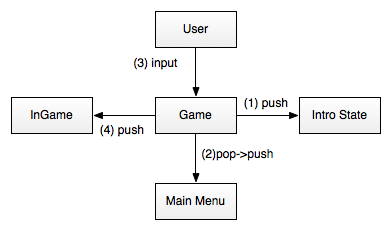
\includegraphics[scale=0.75]{graphics/scenario_1_StartingGame}
	\end{center}
        \caption{Game is started}
\end{figure}

Scenario 1 details which components that interact when a game is started. Scenario
2 details what takes place once a player dies, and achieves a new highscore.

\begin{figure}[H]
	\begin{center}
		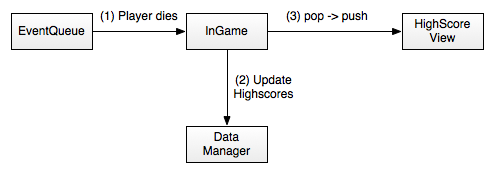
\includegraphics[scale=0.75]{graphics/scenario_2_PlayerDiesHighScore}
	\end{center}
        \caption{Player dies, and achieves a highscore}
\end{figure}
